
This section describes some of the main aspects of the software development
process and software lifecycle as specified in CENELEC EN 50128 and discusses
some potential issues with the implementation using agile methods like SCRUM.

In the openETCS proposal, it was decided to use the V-model for development
(V2.2 Section 3.4.3), as shown in CENELEC EN 50128 Figure~4.

\begin{figure}[ht]
  \centering
  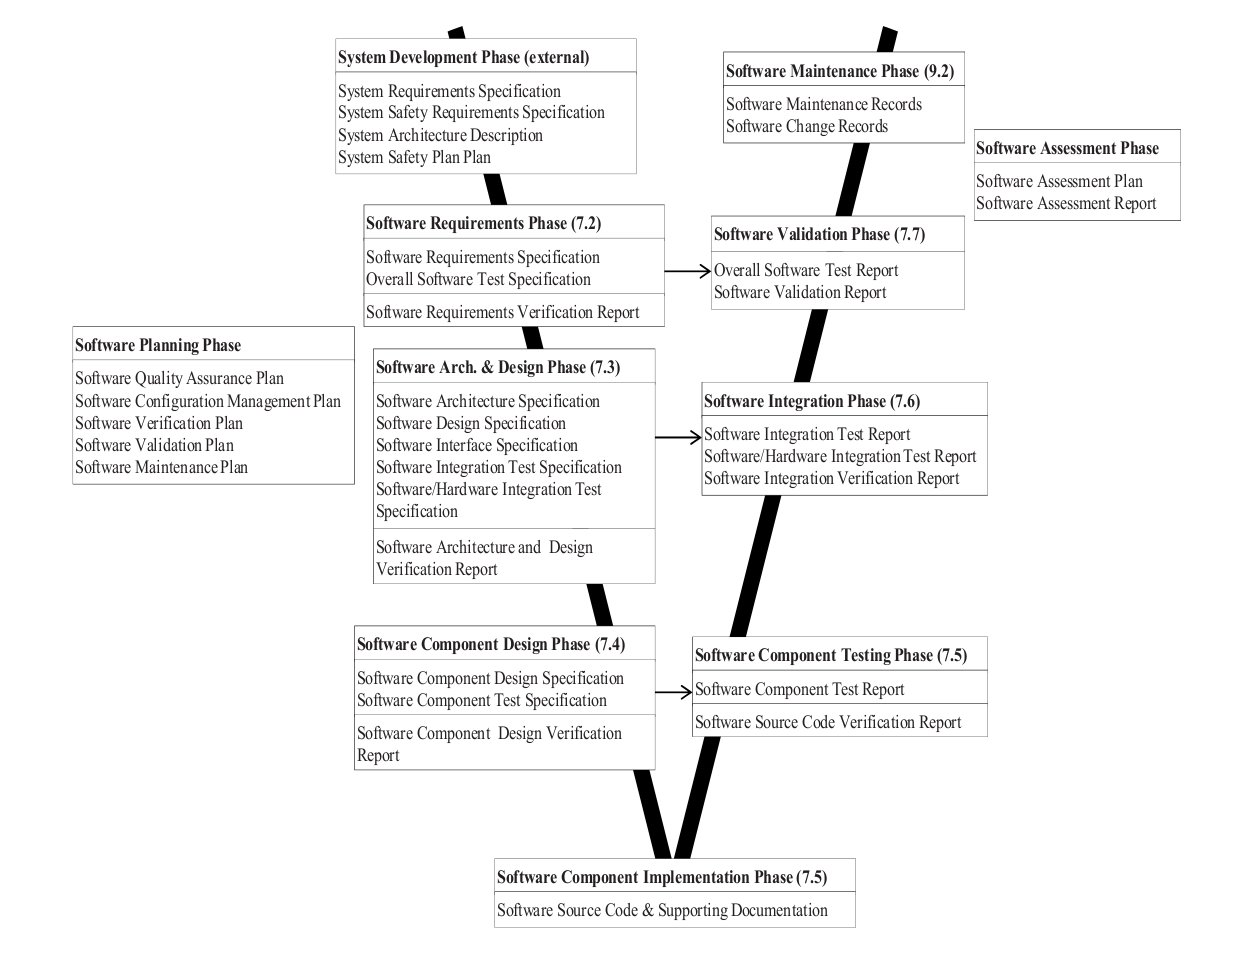
\includegraphics[width=.9\textwidth]{V-Model}
  \caption{General Development Lifecycle as in CENELEC}
  \label{fig:develop-lifecycle-cenelec}
\end{figure}

\subsection{Objectives}
\label{sec:objectives}

The two most important goals of the SW development lifecycle model of CENELEC EN
50128 standard are the separation of the lifecycle into well-defined phases and
the focus on the production and recording of all documentation of the
development process. In addition, the standard specifies some important
constrains which must be fulfilled.

\subsection{Organisational Structure and Roles}
\label{sec:organ-struct-roles}

CENELEC EN 50128 defines a set of required roles for the development of SIL4 (or
SIL3) compliant software (e.g. requirements manager, assessor, etc., for a full
list see 5.1 of CENELEC EN 50128). Theses roles and which of these roles can be
filled by the same person are specified in 5.1.2.10 of the standard. This
distribution and in particular the required separation of several of the roles
will be mandatory for the development process.

\begin{figure}[ht]
  \centering
  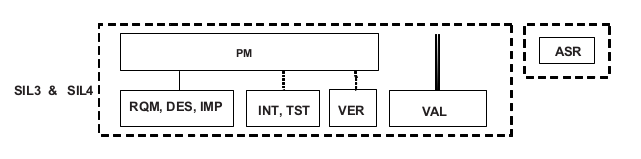
\includegraphics[width=\textwidth]{CenelecRoles}
  \caption{Preferred Organisational Roles}
  \label{fig:preferred-roles}
\end{figure}

Fig.~\ref{fig:preferred-roles} shows the preferred organisational structure
according to CENELEC EN 50128, in particular  the role separations,
e.g., the verifier cannot be the same person as tester, the requirements
manager must be a different person than the integrator and the validator must be
independent of the project manager.

In contrast, the SCRUM development process only defines three roles: project
owner, SCRUM master and team member. These roles mus be refined for an agile SW
development in accordance with the standard.

\subsection{Documentation}
\label{sec:documentation}

The development according to CENELEC EN 50128 is document-centered and many
mandatory documents mus be created. This is in contrast to the agile
development, where only the software is seen as the relevant product. So for
each of the small iterations of the agile process not only the SW shall be of
concern, but also the generated documentation, in particular the update of
existing documentation and the verification of consistency regarding related or
referenced documents.

\subsubsection{Consistency of Documentation}
\label{sec:cons-docum}

It is mandatory to have a consistent definition and usage of all terms,
abbreviations etc. This is especially important if the development process uses
small scale iterations, as the consistency must be assured and restores in
necessary after each iteration. In particular, it must be assured at all times,
that dependent documents, i.e., in hierarchical relation do not contradict each
other.

\subsubsection{Traceability of Requirements}
\label{sec:trac-requ}

For each of the generated documents, the traceability must be assured by
referencing all other concerned documents and by specifying unique reference
numbers. Just like consistency, this traceability is a very important aspect
which is often not a concern in more general software development processes.


\subsection{Quality Assurance}
\label{sec:quality-assurance}

The SW development according to CENELEC EN 50128 requires parallel quality
assurance procedures. This will be well implementable using agile development
which uses several techniques to assure the quality of the results. The test
driven approach and the unit tests used by agile methods, as well as techniques
for increasing code quality like continuous build and pair programming shall be
encouraged.

\subsection{Support Tool Usage}
\label{sec:tool-usage}

Tools to support the development process are classified into three different
classes: T1 for tools which generate no output which any direct or indirect
effect on the resulting code, T2 for tools which support test or verification of
designs or executable code where the tool may fail to indicate errors but cannot
influence the executable code and T3 for tools which may directly or indirectly
influence the code or data of the SW for the safety related system.

The selected tools shall be able to cooperate in the sense that the output of
one tool is usable as input for another tool. The usage of tools of the classes
T2 and T3 must be justified by giving evidence that erroneous can be
detected. It is possible to replace manual tasks by automatization using tools,
in this case evidence for the appropriateness of the tools must be delivered.


%%% Local Variables:
%%% mode: latex
%%% TeX-master: "wp-2.2"
%%% End:
